%% SINH TỰ ĐỘNG từ main.tex — đừng sửa tay.
%% Phần khai báo chép nguyên từ main.tex (chỉ đổi pagestyle và thêm gói float),
%% thân file là mọi khối table/figure của bài, mỗi khối một trang.
%% Dựng lại: xem paper/vcl2026/README.md mục 'Dựng lại bộ ảnh'.
%% VCL2026 -- Hội thảo Quốc gia lần 4 về Ngôn ngữ học Tính toán
%% Bố cục dựng theo ĐÚNG file "VCL_Conference_Paper_Template for authors.docx"
%% (bản chính thức ban tổ chức phát cho tác giả; thông số đọc trực tiếp từ XML của file đó):
%%   khổ A4 · lề 2,54 cm CẢ BỐN PHÍA · Times New Roman 12
%%   giãn dòng 1,5 ở thân bài (theo thông báo hội thảo; template ghi "đôi" -- xem README)
%%   tóm tắt · trích dẫn khối · bảng · tài liệu tham khảo: giãn ĐƠN
%%   thụt đầu dòng 0,5 inch = 36pt · cách đoạn trước 0pt, sau 6pt
%%   nhan đề đậm 14 canh giữa · tác giả nghiêng canh giữa, nối tên cuối bằng "&"
%%   mục cấp 1: SỐ Ả RẬP "1." đậm CANH GIỮA · cấp 2 "1.1." đậm-nghiêng canh trái
%%   cấp 3 "1.1.1." nghiêng canh trái
%%   bảng kiểu APA: KHÔNG kẻ dọc, chỉ ba đường ngang; nhan đề đặt TRÊN bảng,
%%     "Bảng n" đậm ở dòng riêng rồi tiêu đề nghiêng ở dòng dưới, canh trái
%%   ghi chú bảng đặt dưới, cỡ 9
%%   tài liệu tham khảo: APA 7th, xếp theo bảng chữ cái, THỤT TREO 0,5 inch, sang trang mới
%%   cuối bài: Bionote + thông tin liên hệ theo quy định hội thảo
%% DỰNG: tectonic -X compile main.tex --outdir . --keep-logs   (máy này KHÔNG có xelatex)
\documentclass[12pt,a4paper,onecolumn]{article}

%% ---------------- FORMAT (đổi ở đây nếu CFP đổi) ----------------
\usepackage[a4paper,margin=2.54cm,headheight=15pt,headsep=13pt,footskip=1.15cm]{geometry}
\usepackage{fontspec}
\setmainfont{texgyretermes}[
  Extension = .otf, UprightFont = *-regular, BoldFont = *-bold,
  ItalicFont = *-italic, BoldItalicFont = *-bolditalic ]
\setsansfont{texgyreheros}[
  Extension = .otf, UprightFont = *-regular, BoldFont = *-bold,
  ItalicFont = *-italic, BoldItalicFont = *-bolditalic ]
\setmonofont{texgyrecursor}[
  Extension = .otf, UprightFont = *-regular, BoldFont = *-bold,
  ItalicFont = *-italic, BoldItalicFont = *-bolditalic, Scale = MatchLowercase ]
\usepackage{setspace}
\setstretch{1.5}
\setlength{\parindent}{36pt}
\setlength{\parskip}{6pt plus 1pt minus 1pt}
\emergencystretch=1.2em  % tránh tràn lề ở các chuỗi mã dài

%% -- template KHÔNG có tiêu đề chạy trang; chỉ giữ số trang ----------
\usepackage{fancyhdr}
\pagestyle{empty}
\fancyhf{}
\fancyfoot[C]{\fontsize{12}{14}\selectfont\thepage}
\renewcommand{\headrulewidth}{0pt}
\renewcommand{\footrulewidth}{0pt}
%% ---------------------------------------------------------------

\usepackage{polyglossia}
\setmainlanguage{vietnamese}
\setotherlanguage{english}
\usepackage{amsmath}
\usepackage{graphicx}
\usepackage{float}
\usepackage{tikz}
\usetikzlibrary{positioning,arrows.meta,fit,calc}
%% ba màu dùng trong Hình 2, khớp đúng giá trị RGB của lớp vẽ trong tệp ảnh
\definecolor{hinhxanhla}{RGB}{34,200,120}
\definecolor{hinhcam}{RGB}{214,140,30}
\definecolor{hinhxanhduong}{RGB}{40,140,215}
\newcommand{\ôvuông}[2]{\tikz[baseline=-0.45ex]{\draw[#1,line width=0.9pt,#2] (0,0) rectangle (0.34,0.18);}}
\usepackage{array}
\usepackage{booktabs}     % bảng kiểu APA: chỉ đường ngang
\usepackage{enumitem}
\usepackage{indentfirst}
\usepackage{url}
\usepackage[hidelinks]{hyperref}
%% DOI: chi ngat dong sau dau gach cheo, khong ngat giua "doi.org"
\def\UrlBreaks{\do\/}
\setlength{\Urlmuskip}{0mu plus 2mu}
\urlstyle{same}

%% -- đánh số mục theo template: cấp 1 số Ả Rập, đậm, CANH GIỮA ---
\renewcommand{\thesection}{\arabic{section}}
\renewcommand{\thesubsection}{\arabic{section}.\arabic{subsection}}
\usepackage{titlesec}
\titleformat{\section}[block]
  {\normalsize\bfseries\centering}{\thesection.}{0.5em}{}
\titlespacing{\section}{0pt}{12pt plus 2pt}{0pt}
\titleformat{\subsection}[block]
  {\normalsize\bfseries\itshape}{\thesubsection.}{0.5em}{}
\titlespacing{\subsection}{0pt}{9pt plus 2pt}{0pt}
\titleformat{\subsubsection}[block]
  {\normalsize\itshape}{\thesubsubsection.}{0.5em}{}
\titlespacing{\subsubsection}{0pt}{9pt plus 2pt}{0pt}

%% -- nhan đề bảng/hình kiểu APA: nhãn ĐẬM dòng riêng, tiêu đề NGHIÊNG
%%    dòng dưới, canh trái, ĐẶT TRÊN bảng/hình -----------------------
\usepackage{caption}
\DeclareCaptionFormat{apa}{\setstretch{1.0}\raggedright\textbf{#1}\par#3\par}
%% template: nhan đề HÌNH canh giữa (style RALs-FigureCaption), khác nhan đề BẢNG canh trái
\DeclareCaptionFormat{apafig}{\setstretch{1.0}\centering\textbf{#1}\par#3\par}
\captionsetup{format=apa, labelsep=none, singlelinecheck=false,
              textfont=it, skip=4pt, belowskip=4pt}
\captionsetup[figure]{format=apafig}
\renewcommand{\tablename}{Bảng}
\renewcommand{\figurename}{Hình}
%% ghi chú dưới bảng: template style RALs-TableNote = 9 pt, giãn đơn
\newcommand{\tablenote}[1]{\par\vspace{2pt}{\setstretch{1.0}\fontsize{9}{11}\selectfont\raggedright\noindent #1\par}}
%% nội dung bảng: template ghi rõ 10 pt (style RALs-APA-Table, sz=20 half-point)
\newcommand{\bangchu}{\fontsize{10}{12}\selectfont}

%% -- tài liệu tham khảo APA 7th: không đánh số, thụt treo 0,5 inch -
\newenvironment{apareferences}{%
  \newpage
  \section*{TÀI LIỆU THAM KHẢO}%
  \setstretch{1.0}%
  \sloppy%
  \setlength{\parindent}{0pt}%
  \setlength{\parskip}{6pt plus 1pt}%
  \begin{list}{}{%
    \setlength{\leftmargin}{36pt}%
    \setlength{\itemindent}{-36pt}%
    \setlength{\listparindent}{0pt}%
    \setlength{\labelwidth}{0pt}%
    \setlength{\labelsep}{0pt}%
    \setlength{\itemsep}{6pt}%
    \setlength{\parsep}{0pt}%
    \setlength{\topsep}{0pt}}%
}{\end{list}}
\newcommand{\apaitem}{\item[]}

\newcommand{\code}[1]{{\small\texttt{#1}}}
\begin{document}
\setlength{\parindent}{0pt}
\begin{table}[H]
\centering\setstretch{1.0}\bangchu

\renewcommand{\arraystretch}{1.25}
\caption{Hai bản phát hành trên Hugging Face và phần thiếu của mỗi bản.}
\label{tab:nguon}
\begin{tabular}{p{5.3cm}p{4.3cm}p{4.6cm}}
\toprule
\textbf{Kho} & \textbf{Có} & \textbf{Thiếu} \\
\midrule
\code{HarrytheOrange/}\newline\code{\ \ parsed\_AndroidControl}
 & câu chỉ dẫn đủ $15.283$ chuỗi; cây trợ năng $99.131$ màn & không có ảnh \\
\code{ckg/AndroidControl}\newline\code{\ \ ParsedWithImages-20k}
 & ảnh màn hình & đã chuyển sang định dạng tác tử nên mất câu chỉ dẫn theo bước \\
\bottomrule
\end{tabular}

\end{table}
\clearpage
\begin{figure}[H]
\centering\setstretch{1.0}
\caption{Đường đi từ một bước thao tác tới dòng nhãn bốn ô, cùng chỗ mà mỗi bộ lọc can thiệp.}
\label{fig:quytrinh}
\begin{tikzpicture}[
  font=\footnotesize,
  node distance=4.5mm,
  ô/.style={draw,rounded corners=2pt,align=left,inner sep=5pt,text width=7.4cm},
  ghi/.style={align=left,inner sep=3pt,text width=5.4cm,font=\scriptsize\itshape,gray!55!black},
  mũi/.style={-{Latex[length=2.2mm]},gray!60},
  đứt/.style={dashed,gray!55,shorten >=1pt}
]
\node[ô,fill=gray!8] (a) {\textbf{Đầu vào của một bước}\\ ảnh màn hình · cây trợ năng · điểm chạm ghi trong đáp án};
\node[ô,below=of a] (b) {\textbf{Xác định phần tử cần chạm}\\ chọn hộp bao nhỏ nhất có chứa điểm chạm};
\node[ô,below=of b] (c) {\textbf{Ô vai trò và ô toạ độ}\\ tên lớp Android quy về một từ; điểm chạm quy về thang $0$ tới $1.000$};
\node[ô,below=of c] (d) {\textbf{Ô tên}\\ lấy chuỗi ở cây trợ năng trước, chuỗi OCR nằm trong hộp bao sau};
\node[ô,below=of d] (e) {\textbf{Ô dấu hiệu phân biệt}\\ chuỗi OCR gần nhất nằm ngoài hộp bao, cách tâm không quá $350$ px, kèm hướng};
\node[ô,below=of e,fill=gray!8] (f) {\textbf{Dòng nhãn}\\ \code{<desc>icon | (no name) | <point>111,903</point> | just above the text “Gmail”</desc>}};

\foreach \x/\y in {a/b,b/c,c/d,d/e,e/f} \draw[mũi] (\x) -- (\y);

\node[ghi,right=6mm of b.east,anchor=west] (nb) {cây trợ năng lồng nhiều tầng nên một điểm chạm nằm trong hàng chục hộp cùng lúc};
\node[ghi,right=6mm of d.east,anchor=west] (nd) {bộ lọc nhãn trợ năng loại $14{,}7\%$ chuỗi ở lát thử; bộ lọc hình học bỏ hộp phủ quá $25\%$ màn; không nguồn nào cho được chuỗi dùng được thì ô tên là \code{(no name)}, gặp ở $22{,}0\%$ bước};
\node[ghi,right=6mm of e.east,anchor=west] (ne) {không có chuỗi nào đủ gần thì luật lùi về mệnh đề duy nhất, trùng tên hoặc đếm; $75{,}3\%$ dấu hiệu tự nó đủ tách};

\draw[đứt] (b.east) -- (nb.west);
\draw[đứt] (d.east) -- (nd.west);
\draw[đứt] (e.east) -- (ne.west);
\end{tikzpicture}
\end{figure}
\clearpage
\begin{figure}[H]
\centering
\caption{Mỏ neo chữ trên một màn hình thật: bốn biểu tượng cùng vai trò, không biểu tượng
nào có tên.}
\label{fig:moneo}
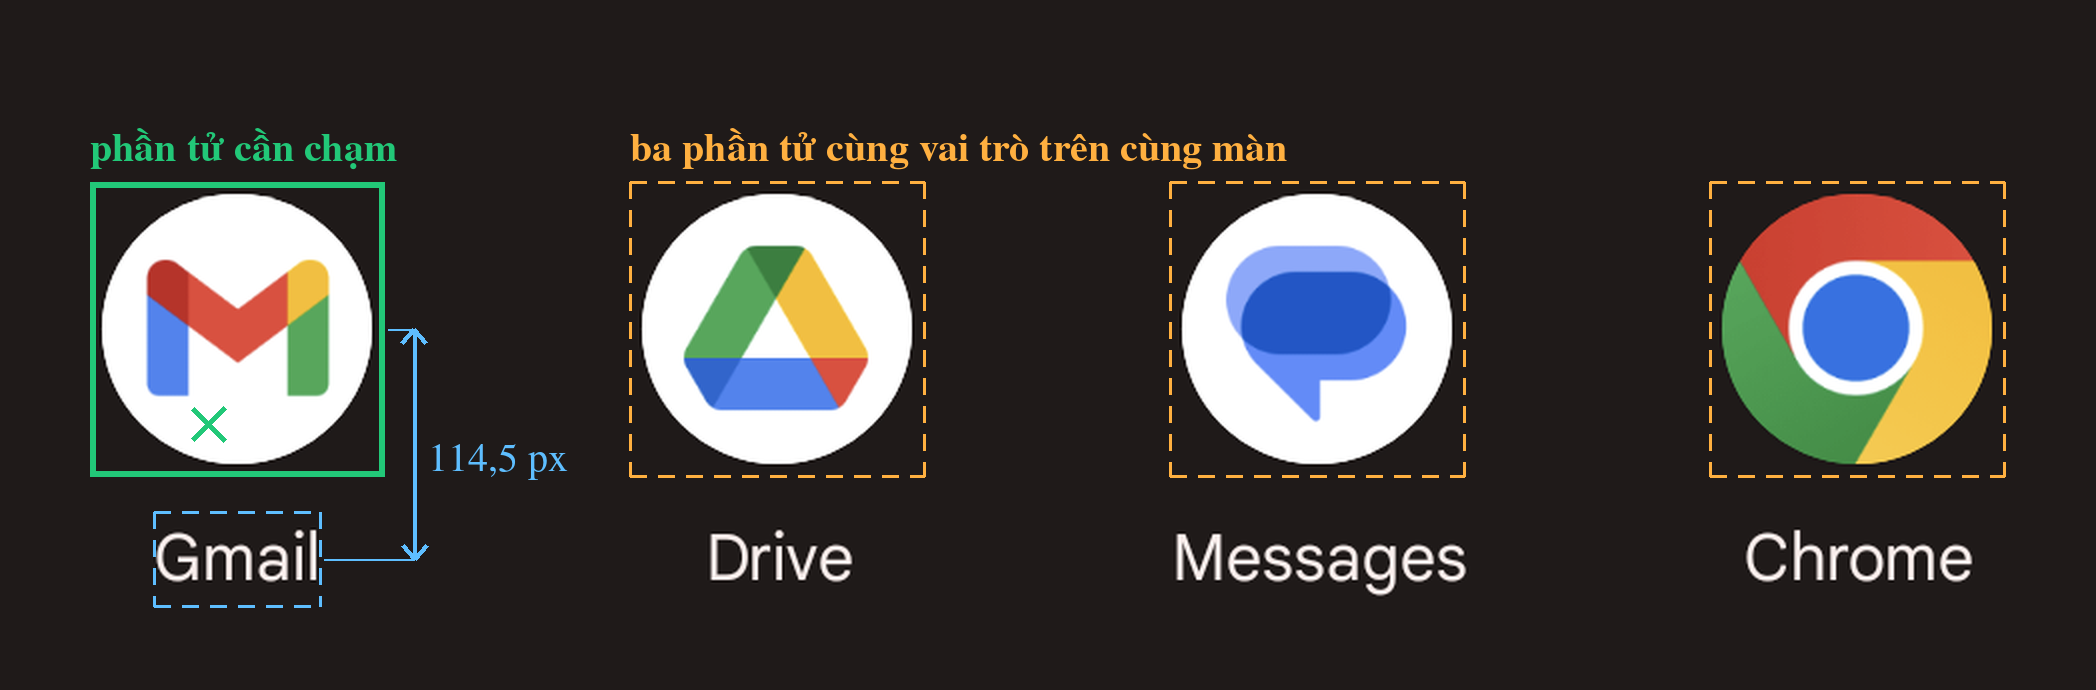
\includegraphics[width=\linewidth]{hinh/fig_moneo.png}

\vspace{5pt}
{\setstretch{1.0}\footnotesize\centering
\code{<desc>icon | (no name) | <point>111,903</point> | just above the text “Gmail”</desc>}\par}

\vspace{5pt}
{\setstretch{1.0}\footnotesize\raggedright\noindent
\textit{Ghi chú.} Ảnh chụp màn hình thật của một bước trong tập kiểm, có phủ thêm lớp vẽ.
Hộp bao, điểm chạm và vị trí chuỗi chữ đều lấy từ cây trợ năng và tệp OCR của chính bước
ấy, nên các khoảng cách trên hình là khoảng cách thật. Khung liền \ôvuông{hinhxanhla}{} là
phần tử cần chạm, còn ba khung nét đứt \ôvuông{hinhcam}{dashed} là ba biểu tượng cùng vai
trò, và không biểu tượng nào trong bốn cái mang tên trong cây trợ năng. Khung nét đứt
\ôvuông{hinhxanhduong}{dashed} là chuỗi OCR gần nhất nằm ngoài hộp bao, cách tâm $114{,}5$
px, nên luật lấy nó làm mỏ neo và sinh ra dòng nhãn ở trên. Câu do người viết cho cùng bước
là \emph{Click on the gmail option}, cũng quy chiếu qua chữ \emph{Gmail}.\par}
\end{figure}
\clearpage
\begin{table}[H]
\centering\setstretch{1.0}\bangchu

\renewcommand{\arraystretch}{1.3}
\caption{Bốn nhãn thật lấy nguyên văn từ tập dạy, kèm câu do người viết cho cùng bước.}
\label{tab:vidu}
\begin{tabular}{p{8.4cm}p{5.6cm}}
\toprule
\textbf{Nhãn tự động} & \textbf{Câu do người viết} \\
\midrule
\code{tappable text | Search here | <point>440,91</point> | just above the text
“Coffee”} & \emph{Click on the search bar} \\
\code{icon | (no name) | <point>256,524</point> | just above the text “Leaf”}
 & \emph{Choose the leaf option} \\
\code{icon | Q | <point>920,899</point> | shares a name with 1 other elements on screen}
 & \emph{click on the search icon} \\
\code{icon | (no name) | <point>920,904</point> | many elements of the same kind on
screen} & \emph{Click on the Right arrow key} \\
\bottomrule
\end{tabular}
\tablenote{\textit{Ghi chú.} Ở hai ca đầu, mệnh đề ở ô thứ tư đủ để chỉ ra phần tử nào là phần tử cần chạm; ở hai ca sau, mệnh đề chỉ cho biết trên màn có phần tử giống nó.}

\end{table}
\clearpage
\begin{table}[H]
\centering\setstretch{1.0}\bangchu

\renewcommand{\arraystretch}{1.2}
\caption{Loại dấu hiệu phân biệt, theo tầng tên của phần tử cần chạm ($41.099$ nhãn).}
\label{tab:hint}
\begin{tabular}{lrrrrr}
\toprule
\textbf{Tầng tên} & \textbf{$n$} & \textbf{Mỏ neo chữ} & \textbf{Duy nhất} & \textbf{Nêu trùng tên} & \textbf{Chỉ đếm} \\
\midrule
Tên rõ ràng   & $30.252$ & $72{,}2\%$ & $7{,}9\%$ & $1{,}7\%$ & $18{,}2\%$ \\
Chỉ có ký hiệu & $1.809$ & $32{,}7\%$ & $4{,}8\%$ & $31{,}3\%$ & $31{,}2\%$ \\
Không có tên   & $9.038$ & $57{,}5\%$ & $9{,}2\%$ & - & $33{,}3\%$ \\
\textbf{Toàn bộ} & $41.099$ & $67{,}2\%$ & $8{,}1\%$ & $2{,}6\%$ & $22{,}1\%$ \\
\bottomrule
\end{tabular}
\tablenote{\textit{Ghi chú.} Hai cột giữa phân giải được mơ hồ, hai cột cuối chỉ nêu sự tồn tại của nó. Tổng hai cột giữa: tầng tên rõ ràng $80{,}1\%$, tầng chỉ có ký hiệu $37{,}5\%$, tầng không có tên $66{,}7\%$, toàn bộ $75{,}3\%$.}

\end{table}
\clearpage
\begin{table}[H]
\centering\setstretch{1.0}\bangchu

\renewcommand{\arraystretch}{1.2}
\caption{Chất lượng nhãn ở quy mô đủ so với lát thử ($n = 1.074$).}
\label{tab:chatluong}
\begin{tabular}{lrr}
\toprule
\textbf{Chỉ số} & \textbf{Quy mô đủ} & \textbf{Lát thử} \\
\midrule
Tên rõ ràng & $73{,}6\%$ & $73{,}8\%$ \\
Chỉ có ký hiệu, không có chữ & $4{,}4\%$ & $2{,}8\%$ \\
Không có tên & $22{,}0\%$ & $23{,}4\%$ \\
Vai trò rõ ràng & $75{,}8\%$ & $76{,}0\%$ \\
Trùng tên trên cùng màn & $7{,}6\%$ & $7{,}0\%$ \\
Có phần tử cùng vai trò để so & $91{,}6\%$ & $92{,}6\%$ \\
\bottomrule
\end{tabular}
\tablenote{\textit{Ghi chú.} Sáu chỉ số đều lệch không quá $1{,}6$ điểm phần trăm giữa hai
quy mô. Mọi chỉ số tính trên bước chạm dựng được nhãn.}

\end{table}
\clearpage
\begin{table}[H]
\centering\setstretch{1.0}\bangchu

\renewcommand{\arraystretch}{1.2}
\caption{Quy mô hai tập sau khi dựng.}
\label{tab:quymo}
\begin{tabular}{lrr}
\toprule
 & \textbf{Tập dạy} & \textbf{Tập kiểm} \\
\midrule
Số bước & $64.567$ & $6.958$ \\
Bước chạm & $41.191$ ($63{,}8\%$) & $4.463$ ($64{,}1\%$) \\
Số tác vụ & $12.895$ & $1.432$ \\
Độ phủ OCR & $100\%$ & $100\%$ \\
Độ phủ nhãn mô tả trên bước chạm & $99{,}8\%$ & $99{,}7\%$ \\
\bottomrule
\end{tabular}

\end{table}
\end{document}
